\section{Dynamical Reputation model}

\begin{figure}[h]
	%%% 6 panels
	%%% columns: Total rep., Mean rep., Number of Active Users
	%%% rows 1: Physics. Theo. Physics, Econ. Beta, Econ. A51
	%%% rows 2: Astro Beta, Astro A51, Lit Beta, Lit A51
	\centering
	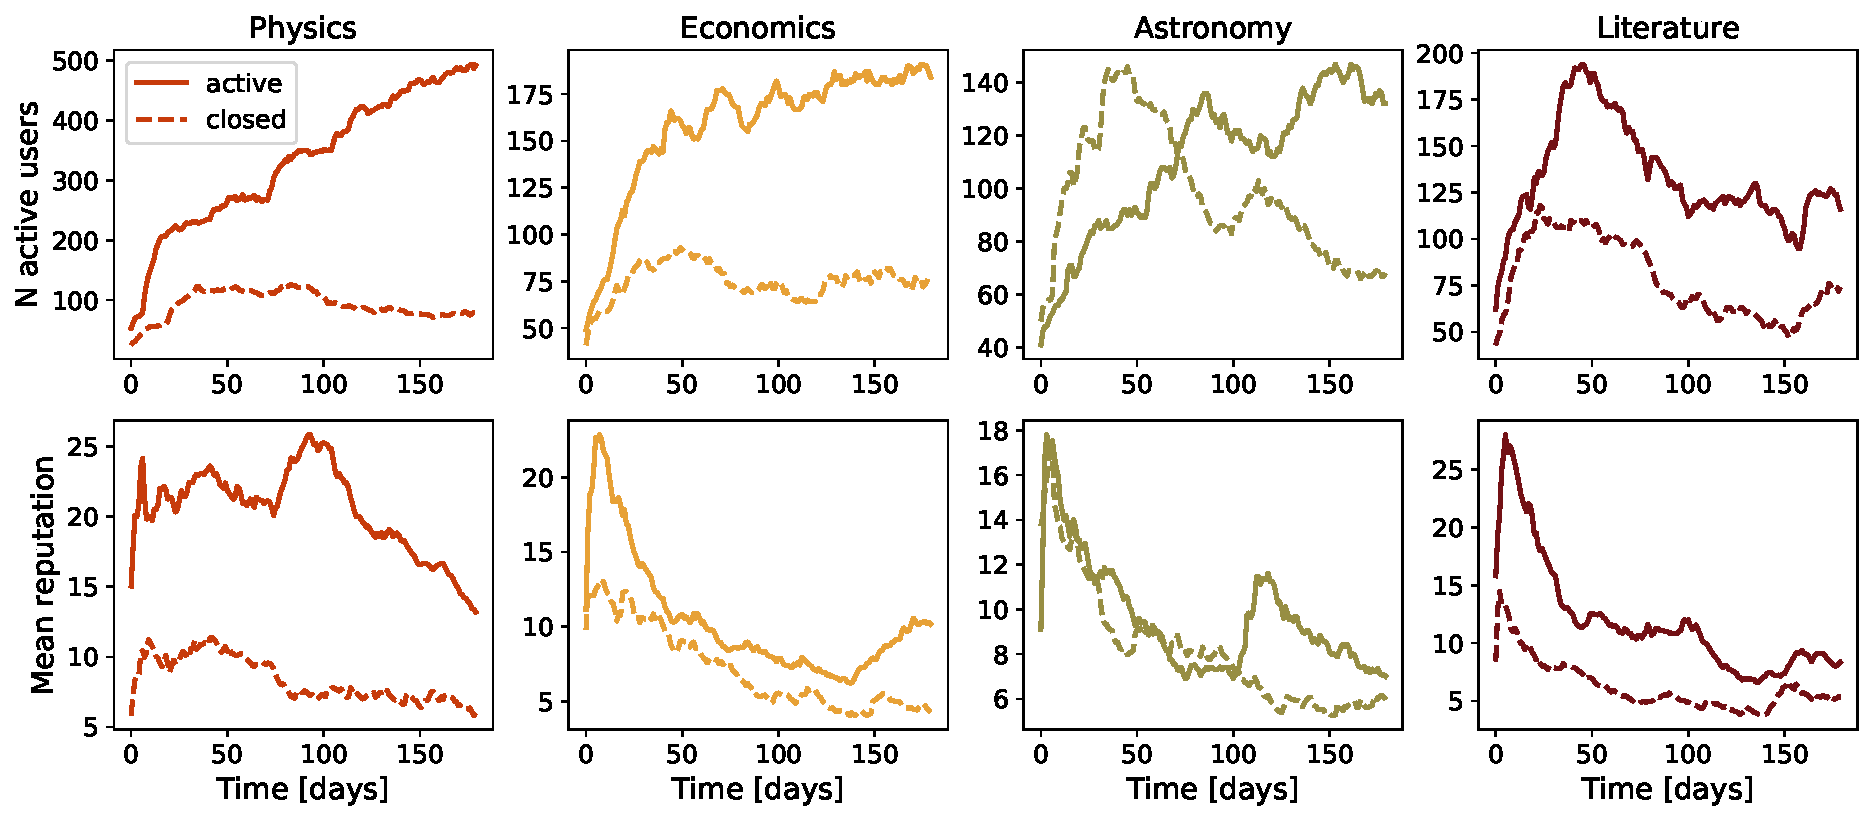
\includegraphics[width=\linewidth]{figures/stackexchange/reputation.pdf}
	\caption{Dynamic Reputation on the four pairs of Stack Exchange websites: Astronomy, Literature, Economics,  Physics and Theoretical Physics.}
	\label{fig:dr6panel}
\end{figure}

\begin{figure}[h]
	\centering
	%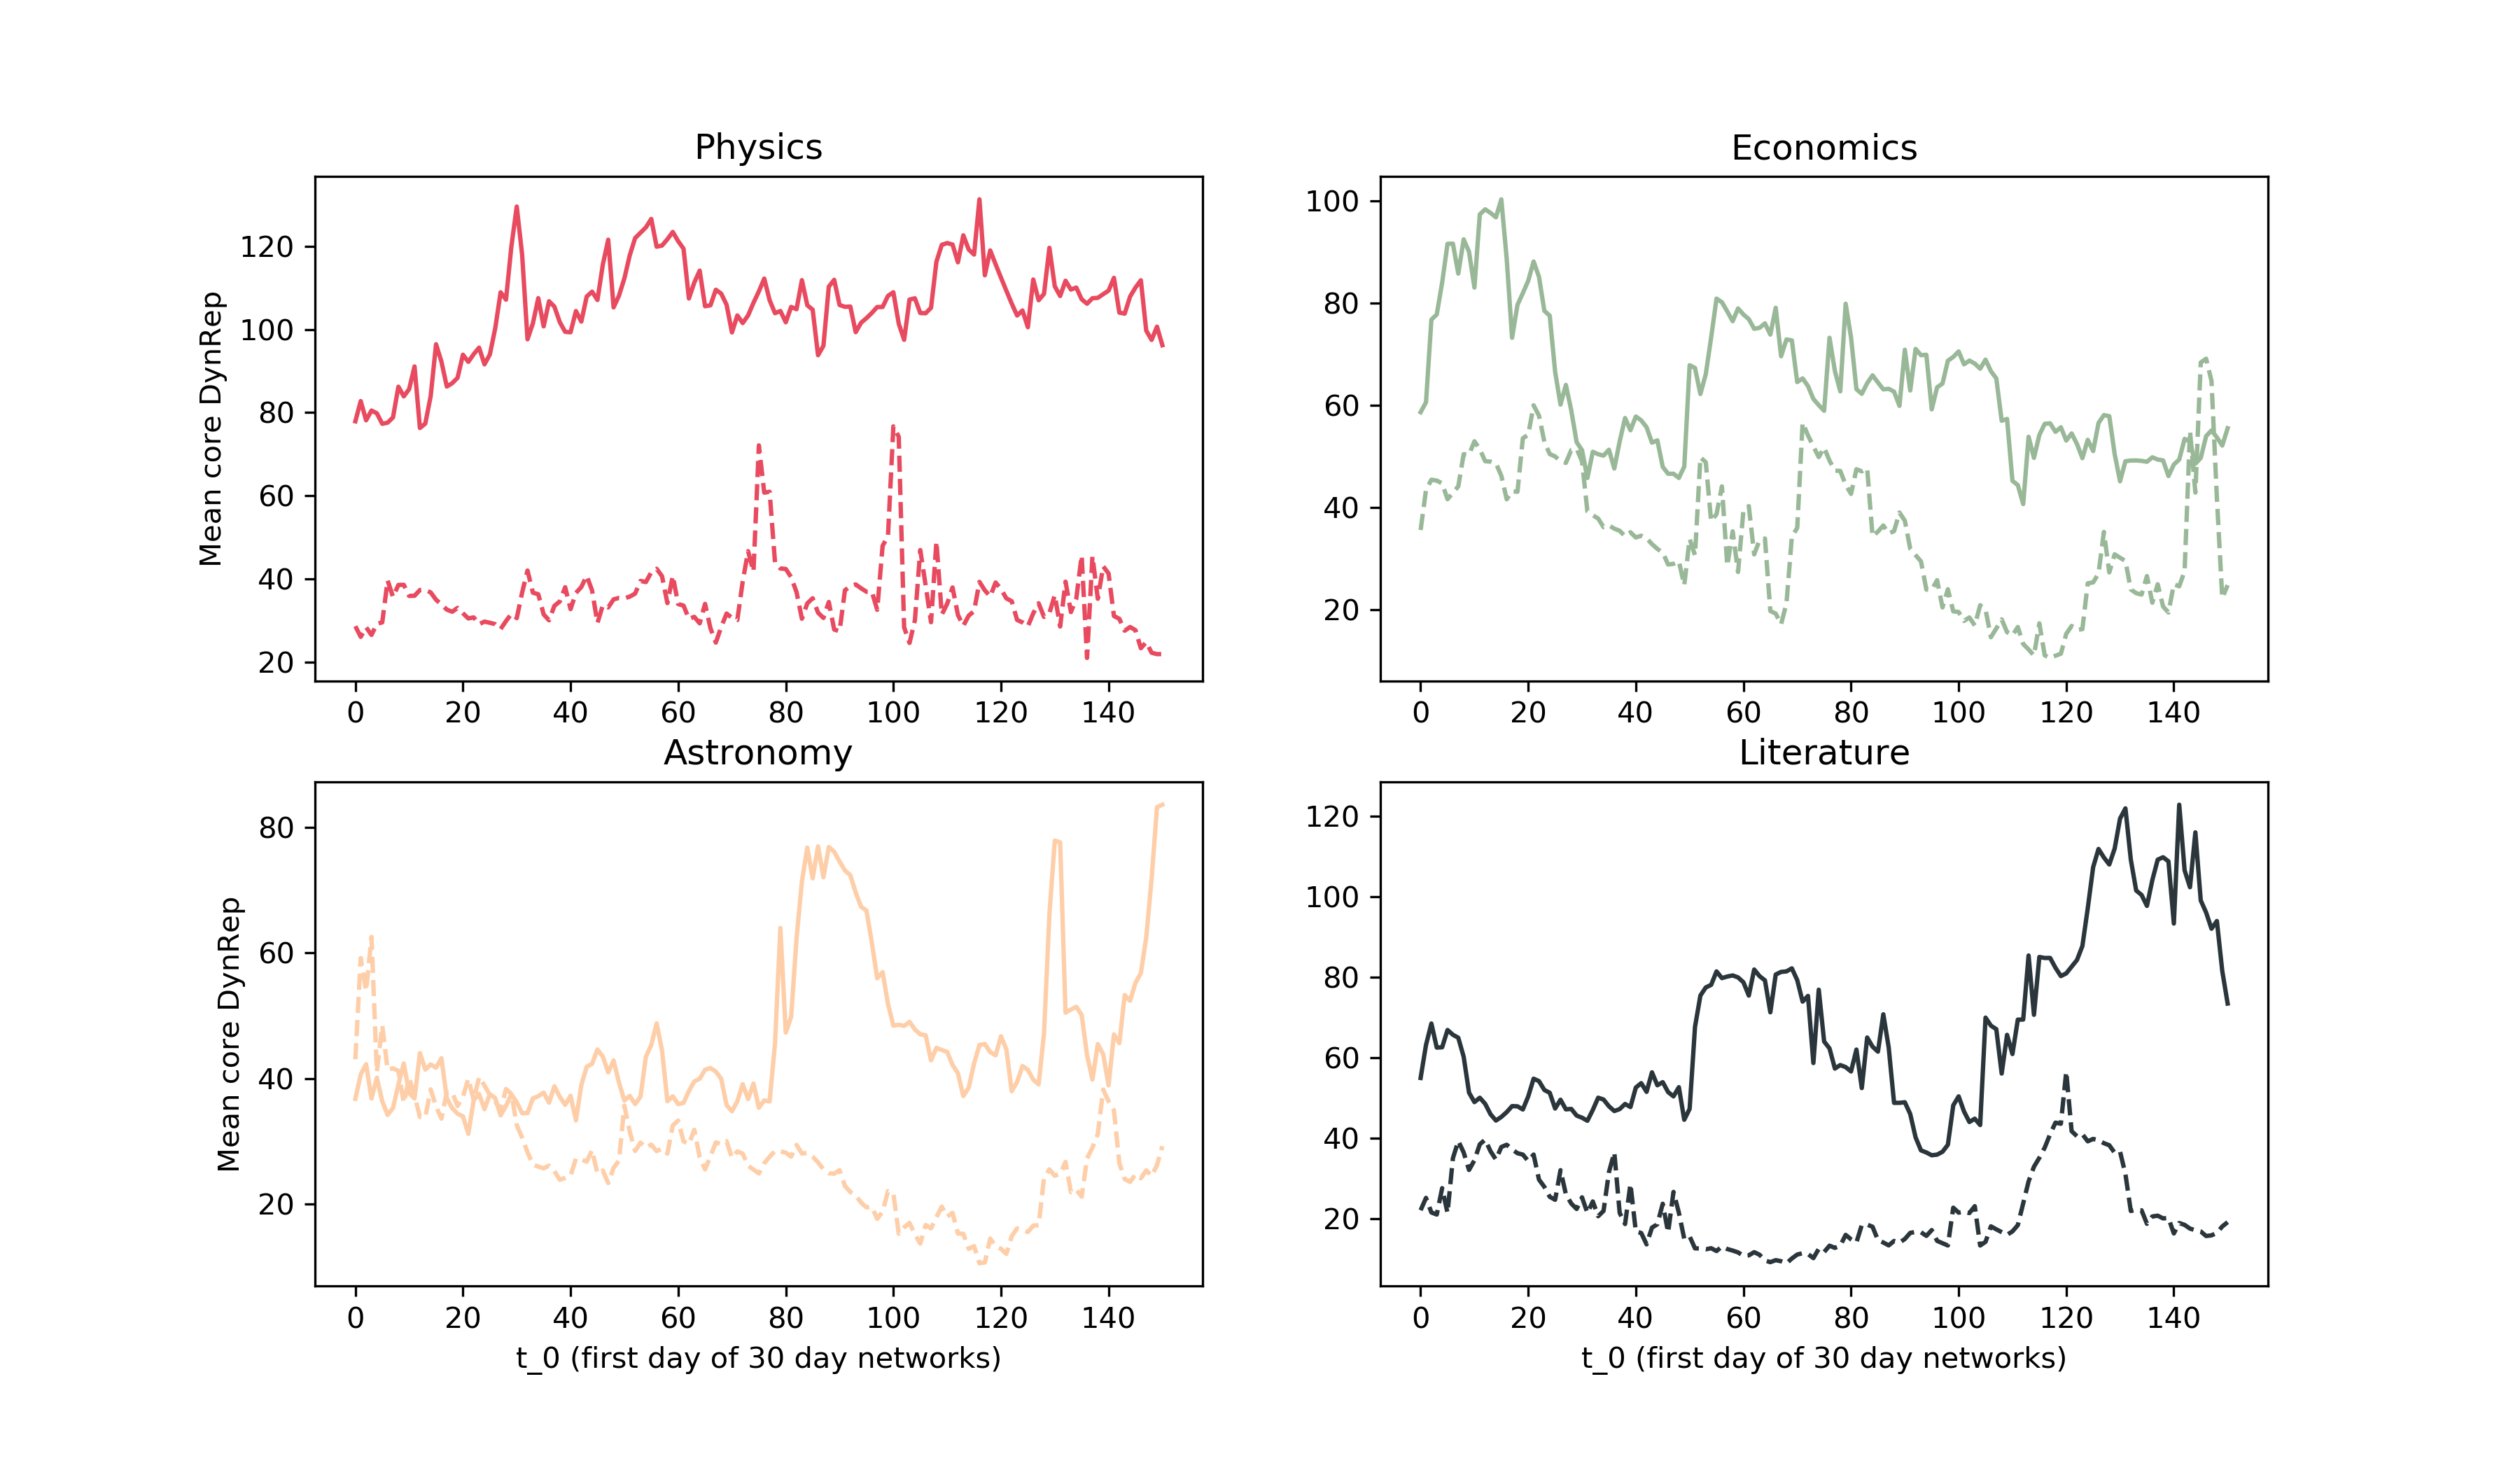
\includegraphics[width=\linewidth]{figures/Mean_core_dyn_rep.png}
	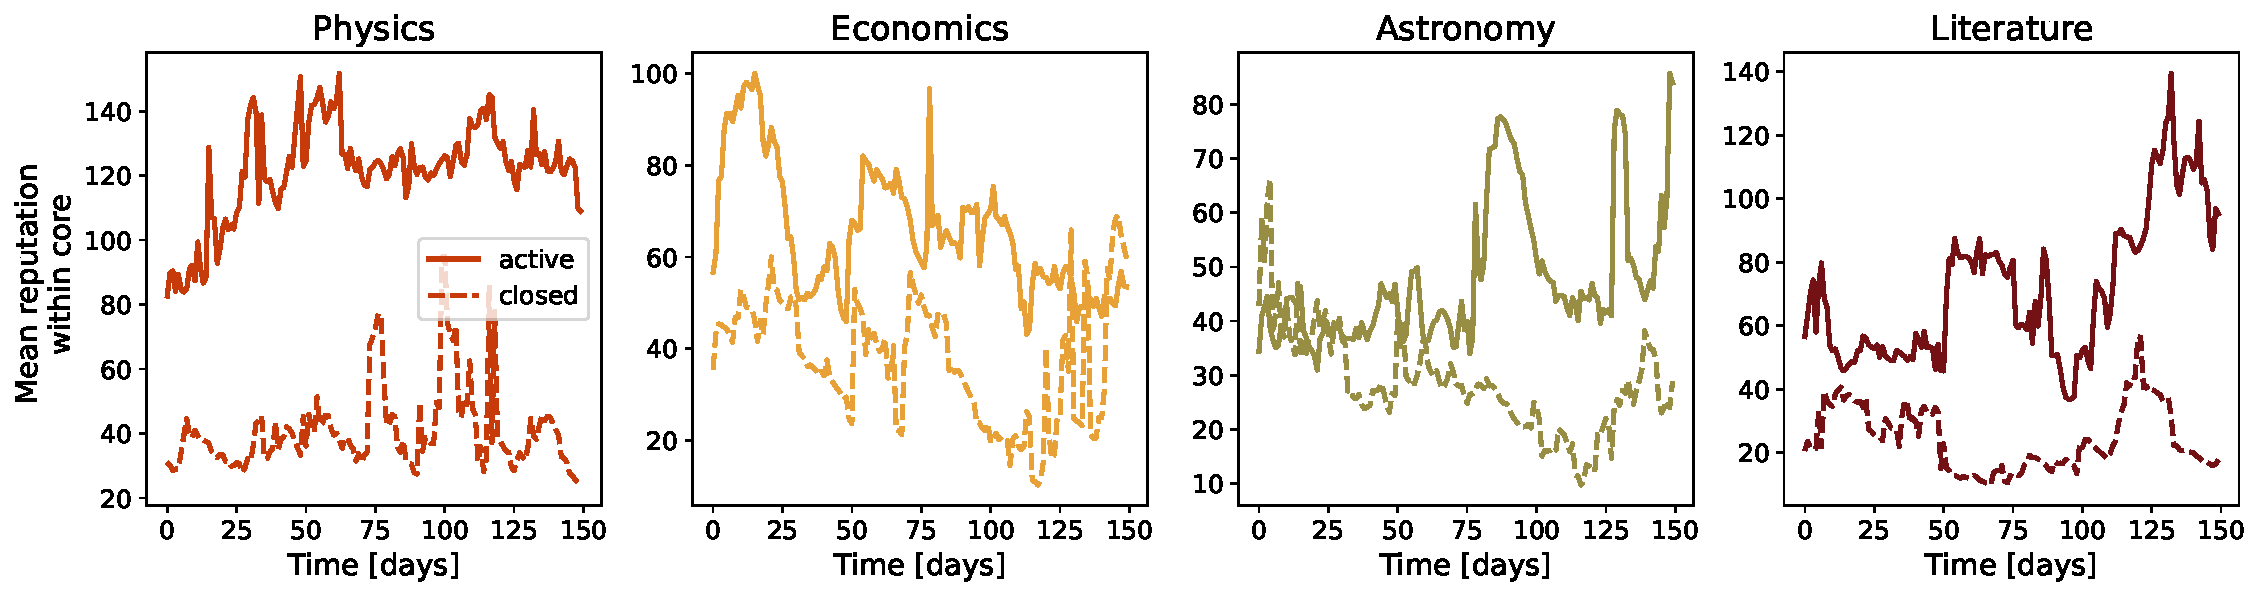
\includegraphics[width=\linewidth]{figures/stackexchange/core_reputation.pdf}
	\caption{Dynamical reputation within core.}
	\label{fig:dr_core}
\end{figure}

%Examined network properties suggest that there are structural differences between active and closed communities. Active communities have higher and more stable local cohesiveness compared to their closed counterparts. The overlap of the set of nodes in the core for active communities shows a significant overlap even for distant subnetworks, meaning that the membership of the core in active communities is more stable.

%To further explore the differences between active and closed communities, we focus on dynamical reputation which is our proxy for collective trust in these communities. We investigate whether and how core-periphery structure is related to collective trust in the network. Figure \ref{fig:dr_core} shows the mean dynamical reputation in the core of active and closed communities and its evolution during the observation period. There are clear differences between active and closed communities when it comes to dynamical reputation. The mean dynamical reputation of core users is always higher in active communities than in closed. As expected, the largest difference is observed between Physics and Theoretical Physics community. The difference between active communities which are still in the beta phase and their closed counterparts is not as prominent, however, the active communities have higher mean dynamical reputation especially in the later phase of community life. The only difference in the pattern is observed for astronomy communities at the early phase of their life, when closed community has a higher value of dynamical reputation than active community. This is in line with similar patterns in the evolution of mean clustering and core-periphery structure. 

%By definition, the core consists of very active individuals and thus we expect higher total dynamical reputation of users in the core in comparison to the the total reputation of users belonging to subnetworks periphery. Figure A12 shows the ratio between the total reputation of core and periphery for closed and active communities and its evolution. The ratio between total reputation of core and periphery in Physics is always higher than in the Theoretical physics community. Similar pattern can be observed for literature communities, although the difference is not as clear as in the case of physics. Ratio of total dynamical reputation between core and periphery is higher for closed community than active one on the economics topic in the early days of community life. However, in the later stage of their lives this ratio becomes higher for active communities. Communities around astronomy topic deviate from this pattern, which once again shows the specificity of these communities. 

%To complete the description of the evolution of dynamic reputation active and closed communities, we examine the evolution of Gini index of dynamical reputation in the whole network which is shown in Fig. A5 in Supplementary Information. The Gini index is always higher for active communities than for closed ones, especially for later times in observation period. Only pattern of Astronomy communities deviates from the pattern observed for other three pairs during the early days. These results indicate that the dynamical reputation is distributed in the population more unequally in the active than in closed communities. The evolution of assortativity coefficient that measures correlations between dynamical reputation of connected users in the subnetworks, shown in Fig. A6, shows that networks are disassortative for the largest part of the observation period. These results suggest that users with high dynamical reputation have tendency to connect with users with low value of dynamical reputation. 


%In Figure~\ref{fig:dyn_rep_coreper} we show mean user reputation in core and in periphery over time (30 day sliding windows as before). We see that the mean user reputation in core is greater in the currently active sites (solid lines, top panels) than in their closed pairs (dashed lines). In the bottom panels, we see that the mean reputation on the network periphery has substantially lower values, and the difference between active and closed sites is less pronounced. 

%For reference in Fig~\ref{fig:core_size} we show core sizes in all sites. We show these in absolute numbers (total number of nodes) and as a fraction of network size through time.

%\textbf{Gini coefficient}
%Besides the number of active users (who at given moment of observation have reputation higher than the threshold) and the population mean value of dynamical reptuation, we have investigated in more details the distribution of dynamical reputation within discussed communities. We have observed that the distributions are often skewed which prompted us to compare the communities in terms of their Gini coefficient. The gini coefficient is a simple measure that shows us the degree of reputation inequality within the community. We calculate the value based on the dynamic reputation values of users at every time step (day) and report he values in Fig.~\ref{fig:dynrep-gini}. We see that all communities (both still active and closed ones) have gini coeffiecinet values higher than $0.5$ throughout first six month period. Interestingly, except in the case of Astronomy, currently active communities had higher reputation inequality every day during first six month period. As in many other measures, in the case of astronomy, closed community started as more unequal one (signalled by higher gini coef values), but after around two months the situation changed. 
\begin{figure}[h!]
	\centering
	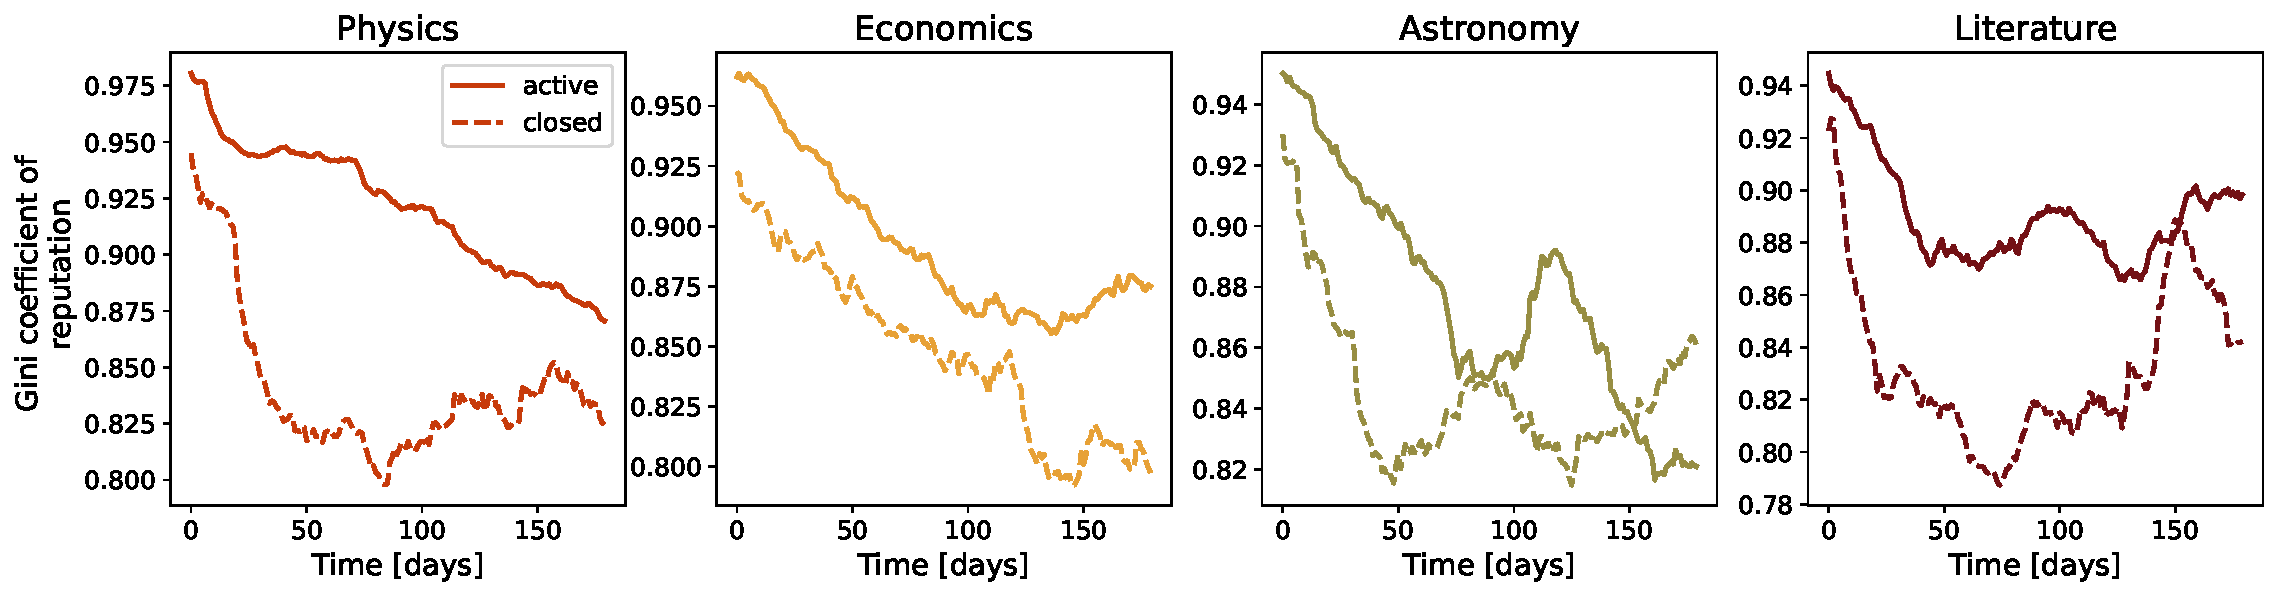
\includegraphics[width=1\linewidth]{figures/stackexchange/gini.pdf}
	\caption{Gini index of dynamic reputation within population}
	\label{fig:dynrep-gini}
\end{figure}

%\subsection{Dynamic reputation in the network of interactions}
%In the few figures below, we investigate whether users' dynamic reputation is related with users' position within the network.

%\textbf{Dynamic Reputation assortativity}

%We first look at user interaction patters, e.g. we investigate whether users connect with others of similar or different reputation (positive/negative assortativity). We operationalize this by measuring assortativity of dynamic reputation on interaction network. Practically this is a meassure of correlation between dynamic reputation of users who are linked in the interaction network. These results are shown in Fig.~\ref{fig:dyn_rep_assort}. We look at 30 day unweighted undirected networks of interactions (questions, answers and comments) and calculate assortativity by using users' reputation on the last day of observed time window. We see small values of assortativity that are mostly negative, signaling weak correlations between reputation levels of interacting users. The fact that the values are mostly negative are expected, users of different dynamic reputation interact, e.g. active, high reputation users respond to the questions of new, less reputable users. Exceptions are closed astronomy and literature sites that occasionally had positive assortativity values, signaling existence of links between users of similar reputation levels.
\begin{figure}[h!]
	\centering
	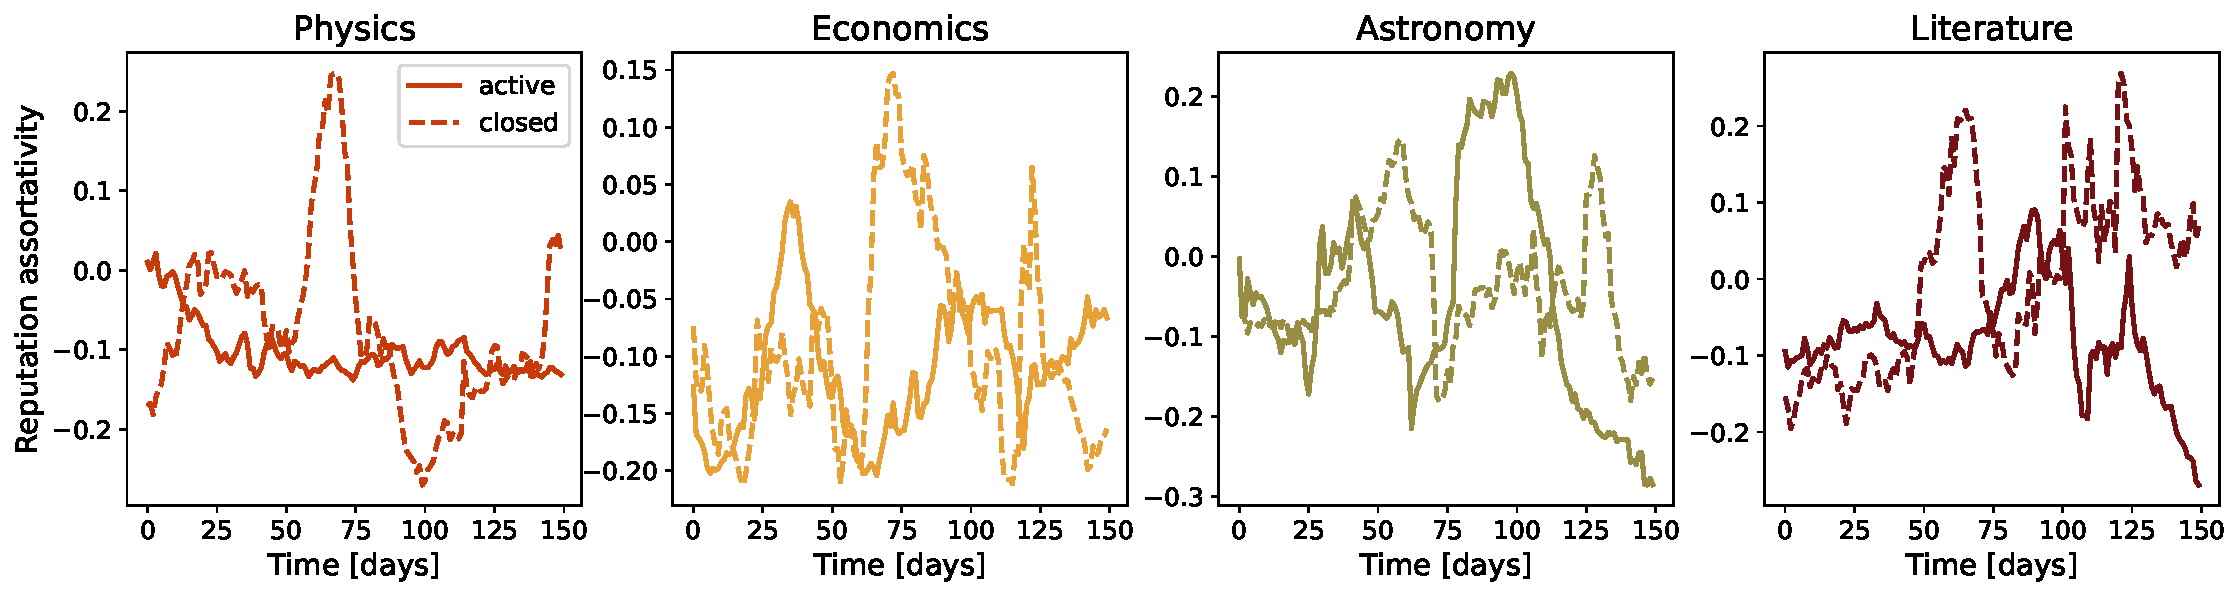
\includegraphics[width=1\linewidth]{figures/stackexchange/reputation_assortativity.pdf}
	\caption{Dynamic Reputation assortativity in the network of interactions (questions, answers, comments, unweighted, undirected network). Solid lines - active sites; dashed lines - closed sites.}
	\label{fig:dyn_rep_assort}
\end{figure}
%% posto se ovo isto gleda na mrezama mozda moze u isti section sa ova dva grafika

%\textbf{DynRep \& Degree}
% dodacu samo korelacije kroz vreme za sad stoji samo placeholder za sliku i opis
%\textbf{DynRep \& BC}
% dodacu samo korelacije kroz vreme

%We continue to investigate whether the user's reputation correlates with typical network centrality measures calculated at user's node in the interaction network. As previously, we compare node's centrality in the 30 day network with the node's dynamic reputation on the last day of the period, repeat the process every day for the first six months. 
%Correlation coefficient between dynamic reputation and degree in the network is very high, as expected, as most of the interactions that contributed to user's reputation are also present as links in the network. We show these results in Fig.~\ref{fig:dyn_rep_centrality}(top). However, we again see the distinction between active and closed communities where this correlation is higher in active communities, except in the first month of sliding windows. Astronomy is an exception here as well as we see that the correlations were similar in both closed and still active sites throughout observed period. 
%There are few steep drops in correlation coefficients in Economics and Literature closed sites, maybe worth further investigation.
%In the bottom panels of Fig.~\ref{fig:dyn_rep_centrality} we present correlation coefficients of dynamic reputation and user's betweenness centrality in the interaction network. These corrlations are also high and most of the time higher in the later networks of active than closed communities. This is particularly interesting due to global nature of betweenness centrality measure and less obvious relation of it to user's dynamic reputation.
\begin{figure}[h!]
	\centering
	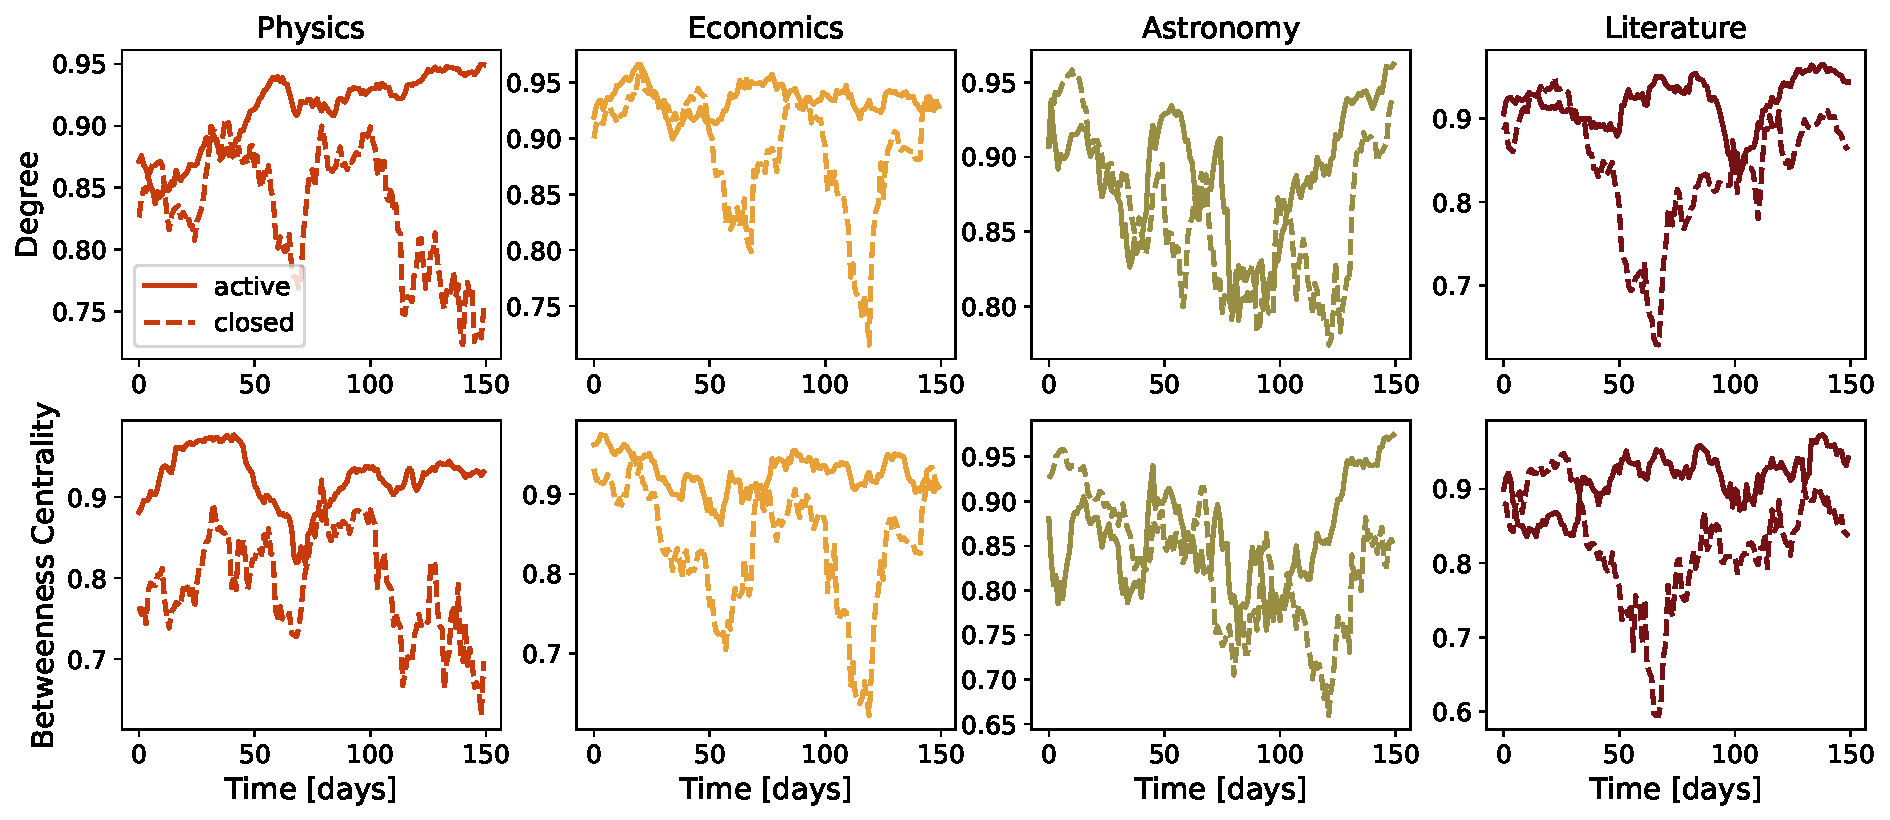
\includegraphics[width=\linewidth]{figures/stackexchange/correlations.pdf}
	\caption{Coefficient of correlation between users' Dynamic Reputation and users' network degree (top) and users's betweenness centrality (bottom). Solid lines - active sites; dashed lines - closed sites.}
	\label{fig:dyn_rep_centrality}
\end{figure}

\begin{figure}[h!]
	\centering
	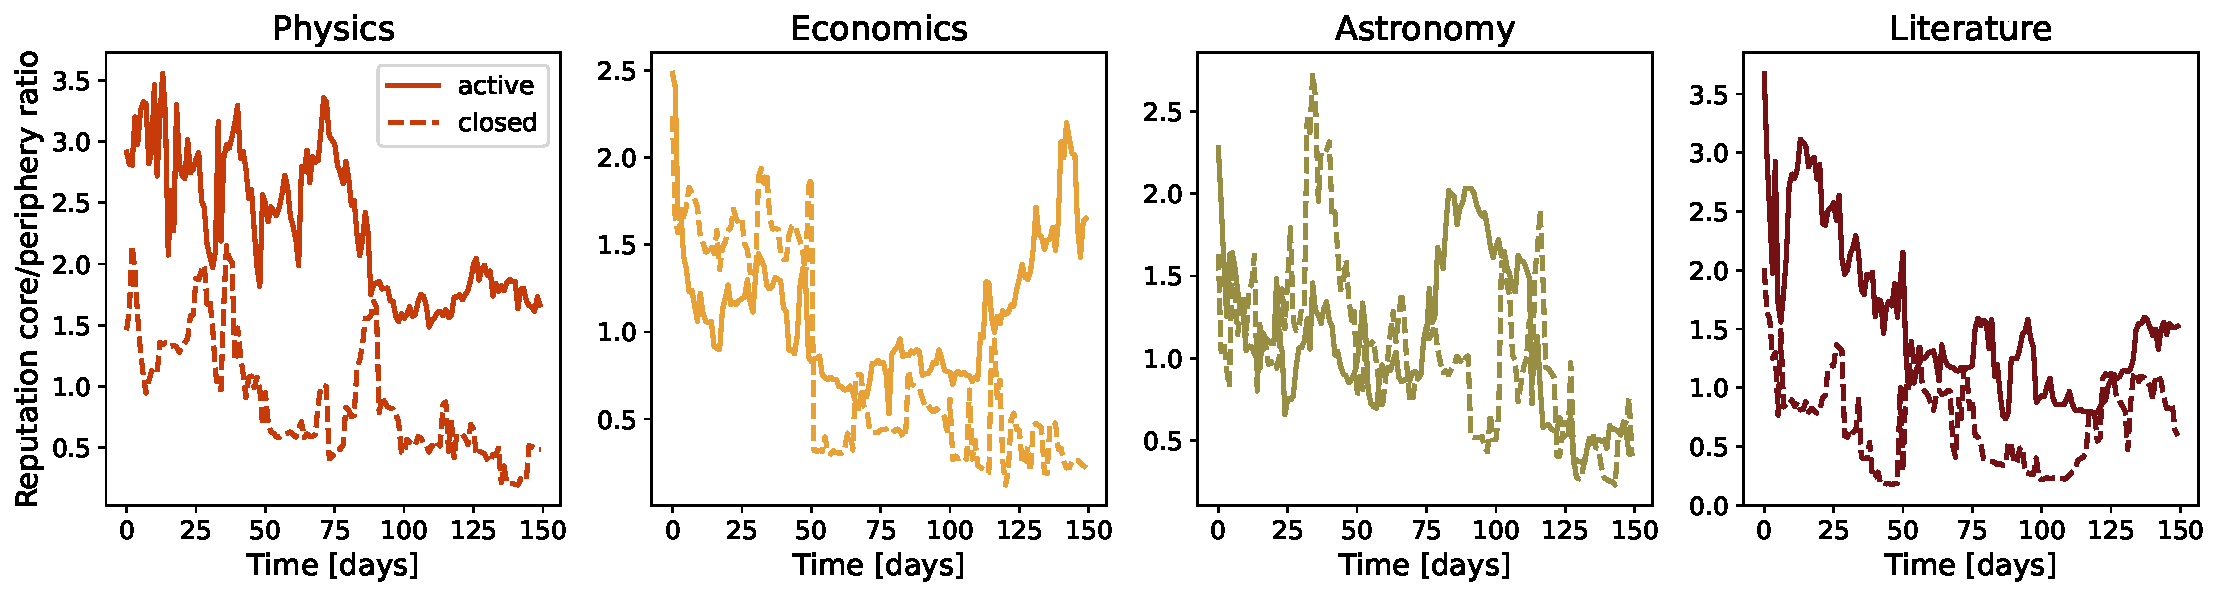
\includegraphics[width=\linewidth]{figures/stackexchange/core_per_ratio_reputation.pdf}
	\caption{Ratio between the total reputation within network core and periphery. Solid lines beta communities, dashed lines area 51 communities.}
	\label{fig:dr_core_per}
\end{figure}
